\documentclass{mc2015}
%
%=================================================================================================
% new commands
% +++++++++++++++++++++++++++++++++++++++++++++++++++++++++++++++++++++++++++++++++++++++++++++++++
\newcommand{\nc}{\newcommand}

% operators
\renewcommand{\div}{\mbold{\nabla}\! \cdot \!}
\newcommand{\grad}{\mbold{\nabla}}
\newcommand{\divv}[1]{\boldsymbol{\nabla}^{#1}\! \cdot \!}
\newcommand{\gradd}[1]{\mbold{\nabla}^{#1}}
\newcommand{\mbold}[1]{\boldsymbol#1}
% latex shortcuts
\newcommand{\bea}{\begin{eqnarray}}
\newcommand{\eea}{\end{eqnarray}}
\newcommand{\be}{\begin{equation}}
\newcommand{\ee}{\end{equation}}
\newcommand{\bal}{\begin{align}}
\newcommand{\eali}{\end{align}}
\newcommand{\bi}{\begin{itemize}}
\newcommand{\ei}{\end{itemize}}
\newcommand{\ben}{\begin{enumerate}}
\newcommand{\een}{\end{enumerate}}
\usepackage{amsthm}
\newtheorem*{remark}{Remark}
% DGFEM commands
\newcommand{\jmp}[1]{[\![#1]\!]}                     % jump
\newcommand{\mvl}[1]{\{\!\!\{#1\}\!\!\}}             % mean value
\newcommand{\keff}{\ensuremath{k_{\textit{eff}}}\xspace}
% shortcut for domain notation
\newcommand{\D}{\mathcal{D}}
% vector shortcuts
\newcommand{\vo}{\mbold{\Omega}}
\newcommand{\vr}{\mbold{r}}
\newcommand{\vn}{\mbold{n}}
\newcommand{\vnk}{\mbold{\mathbf{n}}}
\newcommand{\vj}{\mbold{J}}
\newcommand{\eig}[1]{\| #1 \|_2}
%
\newcommand{\EI}{\mathcal{E}_h^i}
\newcommand{\ED}{\mathcal{E}_h^{\partial \D^d}}
\newcommand{\EN}{\mathcal{E}_h^{\partial \D^n}}
\newcommand{\ER}{\mathcal{E}_h^{\partial \D^r}}
\newcommand{\reg}{\textit{reg}}
%
\newcommand{\norm}{\textrm{norm}}
\renewcommand{\Re}{\textrm{Re}}
\newcommand{\Pe}{\textrm{P\'e}}
\renewcommand{\Pr}{\textrm{Pr}}
%
\newcommand{\resi}{R}
%\newcommand{\resinew}{\tilde{D}_e}
\newcommand{\resinew}{\widetilde{\resi}}
\newcommand{\resisource}{\widetilde{\resi}^{source}}
\newcommand{\matder}[1]{\frac{\textrm{D} #1}{\textrm{D} t}}
%
% extra space
\newcommand{\qq}{\quad\quad}
% common reference commands
\newcommand{\eqt}[1]{Eq.~(\ref{#1})}                     % equation
\newcommand{\fig}[1]{Fig.~\ref{#1}}                      % figure
\newcommand{\tbl}[1]{Table~\ref{#1}}                     % table
\newcommand{\sct}[1]{Section~\ref{#1}}                   % section
\newcommand{\app}[1]{Appendix~\ref{#1}}                   % appendix
%
\newcommand{\ie}{i.e.,\@\xspace}
\newcommand{\eg}{e.g.,\@\xspace}
\newcommand{\psc}[1]{{\sc {#1}}}
\newcommand{\rs}{\psc{R7}\xspace}
%
\newcommand\br{\mathbf{r}}
%\newcommand{\tf}{\varphi}
\newcommand{\tf}{b}
%
\newcommand{\tcr}[1]{\textcolor{red}{#1}}
\newcommand{\tcb}[1]{\textcolor{blue}{#1}}
\newcommand{\mt}[1]{\marginpar{ {\tiny #1}}}

%%%%%%%%%%%%%%%%%%%%%%%%%%%%%%%%%%%%%%%%%%%%%%%%%%%%%%%%%%%%%%%%%%%%%
\usepackage[T1]{fontenc}         % Use T1 encoding instead of OT1
\usepackage[utf8]{inputenc}      % Use UTF8 input encoding
\usepackage{microtype}           % Improve typography
\usepackage{booktabs}            % Publication quality tables
\usepackage{amsmath}
\usepackage{amssymb}
\usepackage{graphicx}
\usepackage{float}
\usepackage[exponent-product=\cdot]{siunitx}
\usepackage[colorlinks,breaklinks]{hyperref}
\hypersetup{linkcolor=black, citecolor=black, urlcolor=black}

\usepackage{lipsum}


\usepackage{color}
\usepackage{caption}
\usepackage{subcaption}
\usepackage{mathrsfs}
% more math
\usepackage{amsfonts}
\usepackage{amstext}
\usepackage{amsbsy}
\usepackage{mathbbol} 


\def\equationautorefname{Eq.}
\def\figureautorefname{Fig.}

%%%%%%%%%%%%%%%%%%%%%%%%%%%%%%%%%%%%%%%%%%%%%%%%%%%%%%%%%%%%%%%%%%%%%
% Insert authors' names and short version of title in lines below

\authorHead{Marc O. Delchini and Jean C. Ragusa}
\shortTitle{Regularization of the non-equilibrium Grey Radiation Hydrodynamic Equations}

%%%%%%%%%%%%%%%%%%%%%%%%%%%%%%%%%%%%%%%%%%%%%%%%%%%%%%%%%%%%%%%%%%%%%
\begin{document}

\title{Regularization of the non-equilibrium Grey Radiation Hydrodynamic Equations with an artificial viscosity method}

\author{Marc O. Delchini}
\author{Jean C. Ragusa}
\affil{
  Department of Nuclear Engineering \\
  Texas A\&M University \\
  College Station, TX 77843 \\
  delchinm@tamu.edu; jean.ragusa@tamu.edu}



\maketitle

\begin{abstract}
In \cite{our_jcp_radhy_paper}, we extended the entropy viscosity method, a viscous regularization to stabilize the numerical solution, 
to the non-equilibrium Grey Radiation-Hydrodynamic equations. 
In this method, the artificial viscosity coefficient is modulated by the entropy production and peaks at shock locations. 
The dissipative terms added by the viscous regularization are consistent with the entropy minimum principle. 
However, the demonstration in \cite{our_jcp_radhy_paper} omitted the relaxation and diffusion terms 
present in the material energy and radiation energy equations. Since then, we have found how to include such terms 
in the derivation of the entropy minimum principle for the regularized non-equilibrium Grey Radiation Hydrodynamic Equations. 
This further strengthens the potential of the entropy viscosity method as a stabilization technique for numerical radiation 
hydrodynamic shock simulations.
\\
%
\emph{Key Words}: radiation-hydrodynamics ; shock-capturing scheme ; entropy viscosity method ; viscous stabilization method.
\end{abstract}

%%%%%%%%%%%%%%%%%%%%%%%%%%%%%%%%%%%%%%%%%%%%%%%%%%%%%%%%%%%%%%%%%%%%%%%%%%%%%
\section{Introduction}\label{sec:intro}
%%%%%%%%%%%%%%%%%%%%%%%%%%%%%%%%%%%%%%%%%%%%%%%%%%%%%%%%%%%%%%%%%%%%%%%%%%%%%
%
Accurately solving the radiation and hydrodynamic equations is the topic of ongoing research. 
Substantial research efforts have focused on Riemann solvers. In
\cite{Balsara},  a Riemann solver is developed for the Radiation-Hydrodynamic equations by considering the frozen approximation 
that uncouples the two physics, radiation and hydrodynamics, components but the validity of such an approximation may be questionable 
in the equilibrium diffusion limit. 
Lowrie et al. \cite{LowrieMorelHittinger} proposed a generalized Riemann solver that accounts for the relaxation terms. 
Edwards and al. \cite{EdwardsMorelLowrie} employed a two-stage semi-implicit IMEX scheme to solve the Radiation-Hydrodynamic equations. 
%A Riemann solver along with a flux limiter is used to resolve shocks and other waves. Their results show good agreement with semi-analytical solutions. 
%
% If one assumes the strong equilibrium diffusion limit in which radiation diffusion is negligible and the radiation simply advects at the material velocity, 
% the radiation hydrodynamics equation can be re-cast in the form of the Euler equations with a radiation-modified equation of state (REOS)  \cite{Woodward}. 
%
In \cite{our_jcp_radhy_paper}, we proposed to solve the non-equilibrium Grey Radiation-Hydrodynamics (GRH) equations by stabilizing the numerical discretization 
using the Entropy Viscosity Method (EVM), developed by Guermond et al. for hyperbolic systems of equations \cite{jlg1, jlg2}. 
%
The EVM is a viscous regularization technique where adequate dissipation terms (viscous fluxes) are added to the governing laws while ensuring 
that the entropy minimum principle holds. Viscosity coefficients modulate the magnitude of the added dissipation such that it is large in shock regions and vanishingly 
small elsewhere. In doing so, shocks can be detected and tracked and an adequate amount of viscosity is added locally to stabilize the numerical scheme. 
Thus, the entropy viscosity coefficients are taken proportional to the entropy production while, at the same time, being bounded from above by a first-order 
viscosity coefficient.
Because of the similarity between Euler equations and the radiation-hydrodynamic equations, we conjectured in \cite{our_jcp_radhy_paper} that the entropy 
viscosity method may be a good candidate for resolving shocks occurring in radiation-hydrodynamic phenomena.

The crux of the EVM lies in satisfying the entropy minimum principle, which states that, at any entropy spatial minimum, the rate of entropy change of a system is equal to or greater than 0. When
adding dissipative terms to the governing laws, one must verify that the entropy minimum principle still holds. Indeed, the functional form of these dissipation terms
is actually chosen such that this principle is verified. In \cite{our_jcp_radhy_paper}, we followed an approach similar to that of \cite{Balsara, LowrieMorel} 
where the relaxation and diffusion terms in the radiation and material energy equations were omitted in order to analyze only the hyperbolic parts of 
the non-equilibrium Grey Radiation-Hydrodynamic equations. Numerical results showed that the functional form of the viscous dissipation hence obtained 
yielded very satisfactory results. 

The aim of this paper is to enhance the theoretical grounds for using the EVM to solve the  Radiation-Hydrodynamic equations by proving that the omitted diffusion
and relaxation terms do not negatively affect the previously obtained dissipative terms. The remainder of the paper is as follows: in \sct{sec:GRH}, we recall
the 1-D non-equilibrium Grey Radiation-Hydrodynamic (GRH) equations. The viscous regularization of the GRH equations based on their hyperbolic parts is recalled in \sct{sec:VR_old}.
In \sct{sec:VR_new}, we demonstrate how that the previous viscous regularization still satisfies the entropy minimum principle when one considers the full GRH equations.
Numerical results are given in \sct{sec:rez}. 

%%%%%%%%%%%%%%%%%%%%%%%%%%%%%%%%%%%%%%%%%%%%%%%%%%%%%%%%%%%%%%%%%%%%%%%%%%%%%
\section{The non-equilibrium Grey Radiation-Hydrodynamic equations}\label{sec:GRH}
%%%%%%%%%%%%%%%%%%%%%%%%%%%%%%%%%%%%%%%%%%%%%%%%%%%%%%%%%%%%%%%%%%%%%%%%%%%%%

The 1-D  non-equilibrium Grey Radiation-Hydrodynamic equations are recalled in \eqt{eq:GRH}:
\begin{subequations}
\label{eq:GRH}
%
\begin{equation}
\label{eq:GRHmass}
\partial_t \left( \rho \right) + \partial_x\left( \rho u \right) = 0 
\end{equation}
%
\begin{equation}
\label{eq:GRHmom}
\partial_t \left( \rho u\right) + \partial_x \left(\rho u^2 + P + \frac{\epsilon}{3} \right) = 0 
\end{equation}
%
\begin{equation}
\label{eq:GRHenerg}
\partial_t \left( \rho E\right) + \partial_x \left[ u \left( \rho E + P \right) \right] = -\frac{u}{3} \partial_x \epsilon - \underline{\underline{ \sigma_a c \left( a T^4 - \epsilon \right) }}
\end{equation}
%
\begin{equation}
\label{eq:GRHrad}
\partial_t \epsilon + \frac{4}{3} \partial_x \left( u \epsilon \right) = \frac{u}{3} \partial_x \epsilon + \underline{\underline{\partial_x \left( \frac{c}{3 \sigma_t} \partial_x \epsilon \right)}} 
+ \underline{\underline{\sigma_a c \left( a T^4 - \epsilon \right)}}
\end{equation}
%
\begin{equation}
\label{eq:EOS}
P = \left( \gamma-1 \right) \rho e
\end{equation}
\end{subequations}
where $\rho$, $u$, $E$, $\epsilon$, $P$ and $T$ are the material density, material velocity, material specific total energy, radiation energy density, material pressure and temperature, respectively. The total and absorption cross sections, $\sigma_t$ and $\sigma_a$, are either constant or are expressed as a function of material density and temperature. The variables $a$ and $c$ are the radiation constant and the speed of light, respectively. The symbols $\partial_t$ and $\partial_x$ denote the temporal and spatial partial derivatives, respectively. 
The material temperature and pressure are computed with the ideal gas equation of state (IGEOS) given in \eqt{eq:EOS} and $e = C_v T$,
where  $e = E - \tfrac 1 2 u^2$ is the specific internal energy. The heat capacity $C_v$ and the heat ratio coefficient $\gamma$ are assumed constant. 
In \eqt{eq:GRH}, we have underlined the diffusion and relaxation terms for future reference.

%%%%%%%%%%%%%%%%%%%%%%%%%%%%%%%%%%%%%%%%%%%%%%%%%%%%%%%%%%%%%%%%%%%%%%%%%%%%%
\section{Viscous regularization of the GRH equations based on their hyperbolic parts}\label{sec:VR_old}
%%%%%%%%%%%%%%%%%%%%%%%%%%%%%%%%%%%%%%%%%%%%%%%%%%%%%%%%%%%%%%%%%%%%%%%%%%%%%

Because the solutions of \eqt{eq:GRH} can develop shocks, dissipative terms are added to each equation to prevent oscillatory behaviors in the numerical solution. 
The presence of these additional terms will modify the entropy residual equation for which we must ensure that the entropy minimum holds. As stated earlier, 
an earlier demonstration omitted the diffusion and relaxation terms present in \eqt{eq:GRH} and only considered the hyperbolic parts of \eqt{eq:GRH}. We briefly reviews these
prior results here.
The hyperbolic portion of the GRH system of equations \emph{with dissipative terms present} on the right-hand side is as follows:
\begin{subequations}
\label{eq:regularized_hyperbolic_GRH}
\begin{equation}
\partial_t \left( \rho \right) + \partial_x\left( \rho u \right) = \partial_x \left( \kappa \partial_x \rho \right) 
\end{equation}
%
\begin{equation}
\partial_t \left( \rho u\right) + \partial_x \left(\rho u^2 + P + \frac{\epsilon}{3} \right) = \partial_x \left( \kappa \partial_x \rho u \right) 
\end{equation}
%
\begin{equation}
\partial_t \left( \rho E\right) + \partial_x \left[ u \left( \rho E + P \right) \right] + \frac{u}{3} \partial_x \epsilon = \partial_x \left( \kappa \partial_x(\rho E) \right)
\end{equation}
%
\begin{equation}
\partial_t \epsilon + \frac{4}{3} \partial_x \left( u \epsilon \right) - \frac{u}{3} \partial_x \epsilon = \partial_x \left( \kappa \partial_x \epsilon \right)
\end{equation}
\end{subequations}
%
where $\kappa$ is a positive and locally defined viscosity coefficient. The functional form of the dissipative viscous fluxes was informed
that the derivation of the entropy residual equation. We provide below the main steps leading to that equation and given in \cite{our_jcp_radhy_paper}.
The same procedure will be followed in \sct{sec:VR_new} when diffusion and relaxation terms are incorporated back in the system of equations. 
Some of the algebraic manipulation may be lengthy and only the final results are provided but no information has been withheld such that the interested
reader should be able to reproduce these results. The entropy function $s$ for the GRH system is assumed to depend upon density $\rho$, internal energy $e$, and radiation 
energy $\epsilon$, i.e., $s( \rho, e, \epsilon)$. Invoking the chain rule
\begin{equation}
\label{eq:app_equ2}
\partial_{\alpha} s = \partial_{\rho} s \partial_{\alpha} \rho +  \partial_{e} s \partial_{\alpha}e +  \partial_{\epsilon} s \partial_{\alpha} \epsilon \,,
\end{equation}
 which holds for any independent variable $\alpha=x,t$, we note that a partial differential equation for the entropy can be obtained. This requires
re-casting  \eqt{eq:regularized_hyperbolic_GRH} in terms of the primitive variables $\rho$ (from  the continuity equation), $u$  (from  the momentum equation),
$e$ (from the total specific energy equation minus the specific kinetic energy equation), and $\epsilon$ (from the radiation energy equation). Note that 
the specific kinetic energy equation is simply obtained by multiplying by $u$ the momentum equation expressed in terms of primitive variables. After some algebra,
the following entropy residual equation is obtained:
%
\begin{equation} \label{eq:app_entr_eq_non_equil}
\rho \frac{Ds}{Dt} = \partial_x \left( \rho \kappa \partial_x s \right) + \kappa \left(\partial_x \rho\right) \left( \partial_x s\right) - \rho \kappa X A X^T  + s_e \rho \kappa (\partial_x u)^2 .
\end{equation} 
% 
where the material derivation notation was used $\frac{Ds}{Dt} := \partial_t s + u \partial_x s$. $X=\left( \partial_x \rho, \partial_x e, \partial_x \epsilon \right)$ and $A$ is the $3 \times 3$ symmetric matrix
 \begin{equation}
 A = 
 \left[
 \begin{array}{ccc}
\rho^{-2}\partial_{\rho} \left( \rho^2 \partial_{\rho} s \right) & \partial_{\rho,e} s & \partial_{\rho} \left( \rho \partial_{\epsilon} s \right) \\
 \partial_{\rho,e} s & \partial_{e,e} s & \partial_{e,\epsilon} s \\
 \partial_{\rho} \left( \rho \partial_{\epsilon} s \right) & \partial_{e,\epsilon} s & \partial_{\epsilon,\epsilon} s
 \end{array}
 \right] .
 \end{equation}
The quadratic form $ X A X^T$ is shown to be negative-definite.
%
The following conditions were assumed to hold:
\begin{subequations}
\label{eq:visc_reg_assumptions}
\begin{equation} \label{eq:visc_reg_assumptions1}
P \frac{\partial s}{\partial e} + \rho^2 \frac{\partial s}{\partial \rho} + \frac{4}{3} \rho \epsilon \frac{\partial s}{\partial \epsilon} = 0 \,,
\end{equation}
%
and the functional form of the entropy is given by
%
\begin{equation}\label{eq:ent_equ}
s( \rho, e, \epsilon) = s_{Euler}(\rho, e) + s_{rad}(\rho, \epsilon) = s_{Euler}(\rho, e)+ \frac{4a^{\tfrac{1}{4}}}{3\rho} \epsilon^{\tfrac{3}{4}} \,.
\end{equation}
\end{subequations}
%
The entropy function is the sum of (i) the entropy for the Euler system of equations $s_{Euler}(\rho, e)$ and (ii) a radiation contribution to the entropy $s_{rad}(\rho,\epsilon)=\tfrac{\beta}{\rho} \epsilon^\frac{3}{4}$. 
$s_{Euler}(\rho, e)$ is concave with respect to the internal energy $e$ and the specific volume $\rho^{-1}$ and is defined through the second law of thermodynamics $Tds_{Euler} = de + P d \rho^{-1}$. $s_{rad}(\rho,\epsilon)$ is concave with respect to the radiation energy density $\epsilon$. 
%

At any spatial position where the entropy is minimum, we have, by definition of the minimum, $\partial_x s =0$ and $\partial_{x,x} s \geq 0$. Therefore, at a minimum, we have $\matder{s}=\partial_t s \geq 0$. Thus, the proposed viscous regularization satisfies the entropy minimum principle for the GRH equations when the diffusion and relaxation terms (underlined in \eqt{eq:GRH} are omitted. In \cite{our_jcp_radhy_paper}, we dealt with the omission of the physical diffusion term $\partial_x( \tfrac{c}{3 \sigma_t} \partial_x \epsilon)$ by noting that the viscous regularization adds its own numerical diffusion term $\partial_x \left( \kappa \partial_x \epsilon \right)$ and we opted to ignore
locally the numerical diffusion term as long as $\frac{c}{3 \sigma_t}$ was larger than the viscosity coefficient $\kappa$. 
%
The effect of the relaxation source terms may need to be investigated in the equilibrium diffusion limit as $\sigma_a c \to \infty$. In this limit, the relaxation source terms behave as dissipative terms and make the system parabolic \cite{Leveque}. 



%%%%%%%%%%%%%%%%%%%%%%%%%%%%%%%%%%%%%%%%%%%%%%%%%%%%%%%%%%%%%%%%%%%%%%%%%%%%%
\section{Entropy minimum principle for the complete GRH equations}\label{sec:VR_new}
%%%%%%%%%%%%%%%%%%%%%%%%%%%%%%%%%%%%%%%%%%%%%%%%%%%%%%%%%%%%%%%%%%%%%%%%%%%%%

In the previous Section, we have reviewed the effect of the viscous regularization on the hyperbolic parts of the GRH equations, where relaxation and diffusion terms have been omitted. Numerical results confirmed that the proposed viscous regularization was behaving properly in the streaming and equilibrium diffusion limits but there was no theoretical justification to explain why the definitions of the dissipative viscous fluxes should remain the same for the complete system of GRH equations. As we demonstrate below, the relaxation and diffusion terms further contribute to the verification of the entropy minimum principle for the full GRH equations with viscous regularization. Since we have already established that the dissipative terms yield the terms shown on the right-hand side of \eqt{eq:app_entr_eq_non_equil}, we omit them in the derivation below since their final functional form will remain unchanged.

Hence, we follow the same procedure as in \sct{sec:VR_old} to establish an entropy equation. First, we start with the full system of GRH equations, \eqt{eq:GRH}, and re-cast it in terms of primitive variables. This becomes
\begin{subequations}
\label{eq:GRH_primitive}
%
\begin{equation}
\label{eq:GRHmass_}
\matder{\rho} + \rho  \partial_x u = 0 
\end{equation}
%
\begin{equation}
\label{eq:GRHmom_}
\rho\matder{u} + \partial_x  P + \frac{1}{3} \partial_x \epsilon = 0 
\end{equation}
%
From \eqt{eq:GRHmom_}, we establish the specific kinetic energy equation:
\begin{equation}
\label{eq:GRH_KE}
\rho\matder{\tfrac{u^2}{2}} + u\partial_x  P +\frac{u}{3} \partial_x \epsilon = 0 
\end{equation}
%
Then, an equation for the specific internal energy (recall that $e=E-\tfrac 1 2 u^2$) is
\begin{equation}
\label{eq:GRHenerg_}
\rho\matder{e}  + \partial_x P = \sigma_a c \left( a T^4 - \epsilon \right) 
\end{equation}
%
The primitive form of the radiation energy equation is:
\begin{equation}
\label{eq:GRHrad_}
\matder{\epsilon} + \frac{4}{3} \epsilon \partial_x u = \partial_x \left( \frac{c}{3 \sigma_t} \partial_x \epsilon \right) + \sigma_a c \left( a T^4 - \epsilon \right)
\end{equation}
\end{subequations}

\noindent
For the next step, we note that (chain rule)
%
\begin{equation}
\rho \matder{s} = \rho \Bigg( s_\rho \matder{\rho} + s_e \matder{e} +s_\epsilon \matder{\epsilon} \Bigg)
\end{equation}
%
and thus linearly combine \eqt{eq:GRHmass_}, \eqt{eq:GRHenerg_}, and \eqt{eq:GRHrad_} to obtain
%
\begin{equation} \label{eq:entro_eq_all_terms}
\rho \matder{s} = \Big( \rho s_\epsilon -s_e \Big)  \sigma_a c \left( a T^4 - \epsilon \right) +   \rho s_\epsilon \partial_x \left( \frac{c}{3 \sigma_t} \partial_x \epsilon \right) 
\end{equation}
%
Note that we invoked \eqt{eq:visc_reg_assumptions1}.
If we can prove that the right-hand side of \eqt{eq:entro_eq_all_terms} is positive, then the proposed viscous regularization, shown in the hyperbolic portion of the GRH equations in \eqt{eq:regularized_hyperbolic_GRH}, will
also be entropy-minimum satisfying for the full GRH equations. 

The right-hand side of \eqt{eq:entro_eq_all_terms} contains two terms which we analyze separately. Using the entropy function given in \eqt{eq:ent_equ}, the first term becomes
\begin{equation} 
\Big( \rho s_\epsilon -s_e \Big)  \sigma_a c \left( a T^4 - \epsilon \right) 
= \left( \left( \frac{a}{\epsilon}\right)^\frac{1}{4} - \frac{1}{T} \right)   \sigma_a c \left( a T^4 - \epsilon \right) 
\end{equation}
Using the identity $(x-1)(x^4-1) = (x-1)^2(x+1)(x^2+1)$, the above equation can be rewritten as
\begin{equation} 
\Big( \rho s_\epsilon -s_e \Big)  \sigma_a c \left( a T^4 - \epsilon \right) 
= \frac{\sigma_a c}{T \epsilon}  (x-1)^2(x+1)(x^2+1) \geq 0
\end{equation}
with $x=  \left(\frac{aT^4}{\epsilon}\right)^\frac{1}{4} \geq 0.$

The second term on the right-hand side of \eqt{eq:entro_eq_all_terms} can be recast by noting that $s_\epsilon = \frac{a^{1/4}}{\rho} \epsilon^{-1/4}$. Rewriting $s_{rad}(\rho, \epsilon) = \frac{4a^{1/4}}{3\rho} \epsilon^{3/4}$ as  $s_{rad}(\rho, \epsilon) = \frac{\tilde{s}_{rad}(\epsilon)}{\rho}$, we have
$ \rho s_\epsilon = \tilde{s}^\prime_{rad}(\epsilon)$. Hence, 
%  \rho s_\epsilon \partial_x \left( \frac{c}{3 \sigma_t} \partial_x \epsilon \right) 
\begin{equation}
\rho s_\epsilon \partial_x \left( \frac{c}{3 \sigma_t} \partial_x \epsilon \right) 
=
 \tilde{s}^\prime_{rad}(\epsilon) \partial_x \left( \frac{c}{3 \sigma_t} \partial_x \epsilon \right) 
\end{equation}
%
Integrating by parts, we obtain
%
\begin{multline} \label{eq:final_form_second_term}
\rho s_\epsilon \partial_x \left( \frac{c}{3 \sigma_t} \partial_x \epsilon \right) 
=
 \partial_x \left(  \tilde{s}^\prime_{rad}  \frac{c}{3 \sigma_t} \partial_x \epsilon \right) 
-
\frac{c}{3 \sigma_t} \left(  \partial_x \epsilon \right)  \left( \partial_x \tilde{s}^\prime_{rad}  \right) \\
=
 \partial_x \left(   \frac{c}{3 \sigma_t} \partial_x \tilde{s}_{rad}  \right) 
-
\frac{c}{3 \sigma_t} \tilde{s}^{\prime\prime}_{rad}  \left(  \partial_x \epsilon \right)^2   \qquad  \qquad  \qquad \ 
\end{multline}
%
The first term in \eqt{eq:final_form_second_term} a conservative term (it only yields boundary terms when integrating over time and space and thus plays no role in entropy production of the system, \cite{Leveque}). The second term  in \eqt{eq:final_form_second_term} is positive 
since $s_{rad}$ (and thus $\tilde{s}_{rad}$) is, by definition, concave with respect to $\epsilon$, i.e., $\tilde{s}^{\prime\prime}_{rad} \leq 0$.

In conclusion, we have 
\begin{equation} 
\rho \matder{s} = \Big( \rho s_\epsilon -s_e \Big)  \sigma_a c \left( a T^4 - \epsilon \right) +   \rho s_\epsilon \partial_x \left( \frac{c}{3 \sigma_t} \partial_x \epsilon \right) \geq 0 \,,
\end{equation}
which demonstrates that the full GRH equations are entropy-minimum satisfying. Consequently, the viscous regularization shown in \eqt{eq:regularized_hyperbolic_GRH} equally applies to the full GRH equations. 

%%%%%%%%%%%%%%%%%%%%%%%%%%%%%%%%%%%%%%%%%%%%%%%%%%%%%%%%%%%%%%%%%%%%%%%%%%%%%
\section{Radiation-hydrodynamic shock results}\label{sec:rez}
%%%%%%%%%%%%%%%%%%%%%%%%%%%%%%%%%%%%%%%%%%%%%%%%%%%%%%%%%%%%%%%%%%%%%%%%%%%%%
%\tcr{at M\&C, they will complaint if we do not show a COMPUTATION. It is the theme of the conference and they check closely for that. So, I will we need to add 1 numerical results. I do not want to copy/paste one from the JCP paper, though we could since the paper has not been published yet....\\}
%
We present 1-D numerical results for a Mach 5 radiative shock test case taken from the published literature \cite{EdwardsMorelLowrie}. The artificial viscosity coefficient $\kappa$ present in the viscous regularization of the GRH is computed using the entropy viscosity method \cite{jlg1,jlg2,our_jcp_radhy_paper}. The governing equations are spatially discretized using continuous linear finite elements and a fully-implicit BDF2 time integrator is employed. The resulting nonlinear equations are solved using a Newton technique to determine the solution values at the end of each time step. The numerical results are obtained with a mesh of $500$ cells and with a Courant-Friedrichs-Lewy (CFL number) of $10$ until steady-state. The boundary conditions for the hydrodynamics equations and radiation equation are considered independently since the latter one is of parabolic nature. For the hydrodynamics equations, we use the following: at the inlet, the flow is supersonic and, therefore, no physical information exits the system. Thus, Dirichlet boundary conditions can be used. At the outlet, the flow becomes subsonic which requires a particular treatment: a static boundary condition is implemented by only specifying the back pressure and computing the other variables from the characteristic equations. For the radiation equation, vacuum boundary conditions are used at both inlet and outlet. \\
%\tcr{can you add some SHORT text for 1 or 2 examples and add a few graphs. For the figures, I would prefer that we use some of your older figures so that they do not look identical tot he JCP paper. The main reason I wanted to write this conference proceedings was to show the results of the JCP paper to the radiation transport community ...}
%
The Mach $5$ test consists of a 1-D slab of thickness $L=0.05$ $cm$, with the initial conditions given in \tbl{tbl:table6}, and is run until a steady state has been reached. The initial discontinuity between the left and right states is located at $x_0 = 0  \ cm$. The opacities $\sigma_t$ and $\sigma_a$ are assumed constant and set to $853.144$ $cm^{-1}$ and $390.711$ $cm^{-1}$, respectively. The heat capacity at constant specific volume is set to $C_v = 0.12348$ $jerks/(g-keV)$ (we recall that 1 $jerks = 10^9\ Joules$). Steady-state results are shown in \fig{fig:Mach5_temp}, \fig{fig:Mach5_dens}, and \fig{fig:Mach5_visc} for the material and radiation temperatures, the density and the viscosity coefficients, respectively. The exact solution is also plotted for comparison and was obtained from a semi-analytical technique.
%
\begin{table}[H]
\caption{\label{tbl:table6} Initial conditions for Mach $5$.}
\begin{center}
\begin{tabular}{|c|c|c|}
\hline 
 & left  & right \\ \hline
$\rho$ $(g/cm^3)$ &$1.$ & $1.0749588$ \\ \hline
$u$ $(cm/sh)$& $0.1405588$ & $0.1083456$ \\ \hline
$T$ $(keV)$& $0.1$ & $0.1194751$\\ \hline
$\epsilon$ $(jerks/cm^3)$ & $1.372$ $10^{-6}$ & $2.7955320$ $10^{-6}$\\
\hline
\end{tabular}  
\end{center}  
\end{table}
%
\begin{figure}[H]
\centering
\begin{subfigure}[b]{0.47\textwidth}
                \centering
                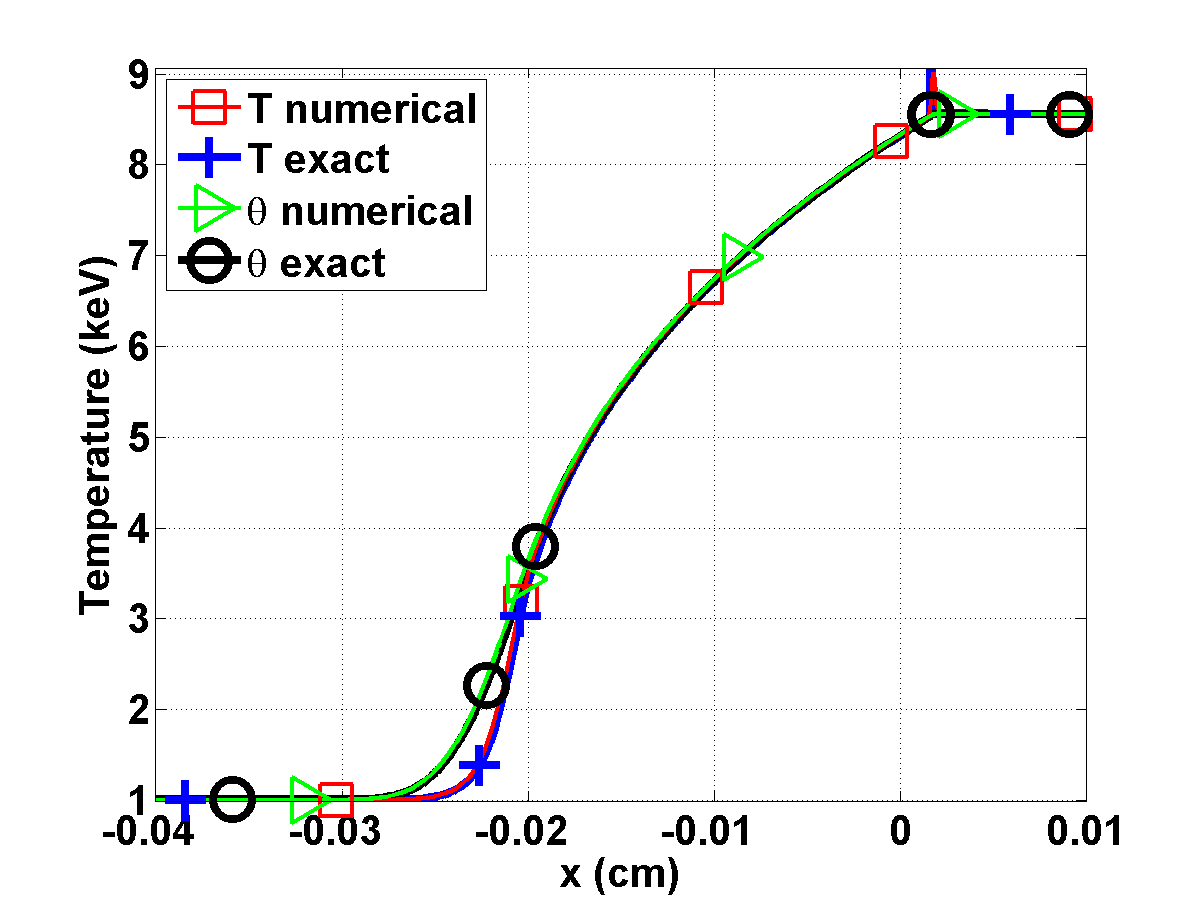
\includegraphics[width=\textwidth]{figs/Mach_5_nel_500_temperature.png}
        \caption{Material and radiation temperature profiles at steady state for the Mach 5 test.}\label{fig:Mach5_temp}
\end{subfigure}
\begin{subfigure}[b]{0.47\textwidth}
                \centering
                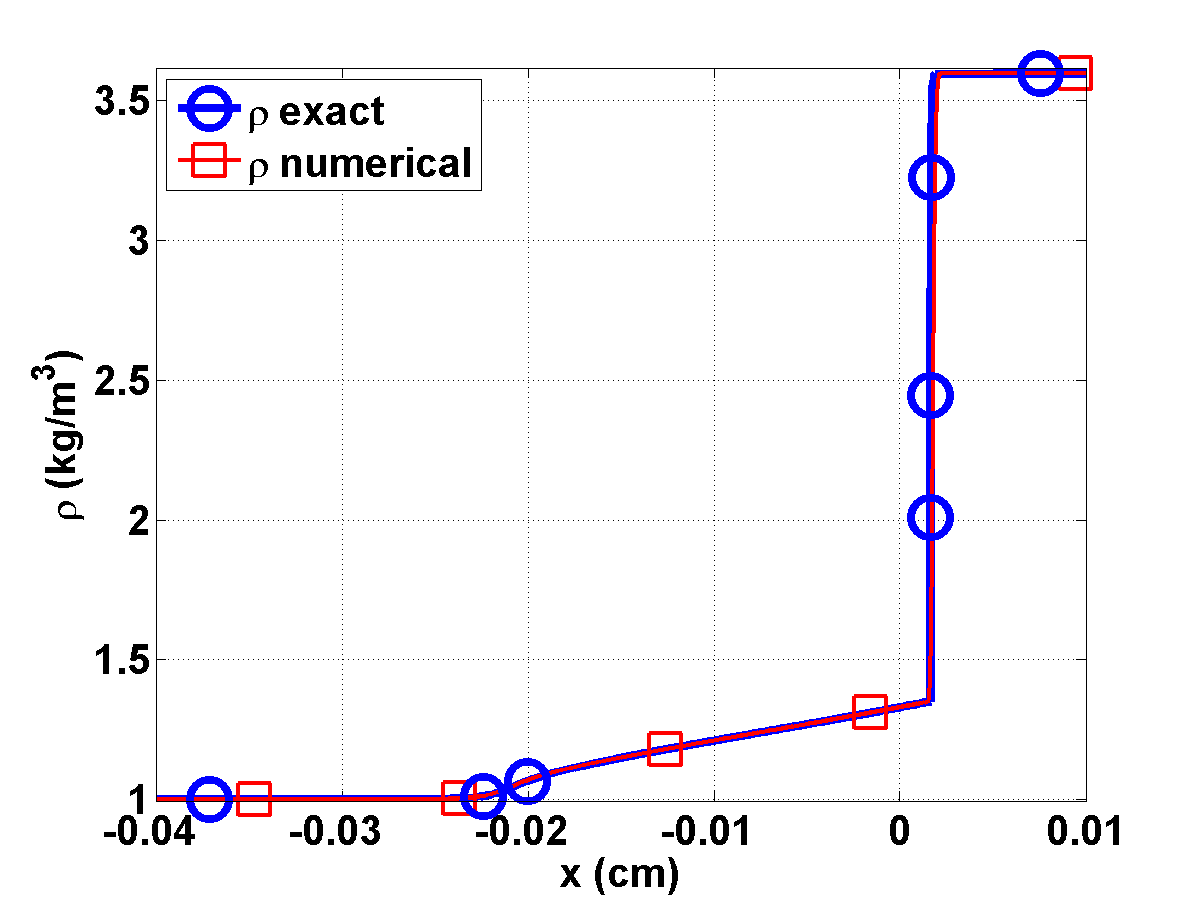
\includegraphics[width=\textwidth]{figs/Mach_5_nel_500_density.png}
        \caption{Density profiles at steady state for the Mach 5 test.}\label{fig:Mach5_dens}
\end{subfigure}
\begin{subfigure}[b]{0.47\textwidth}
                \centering
                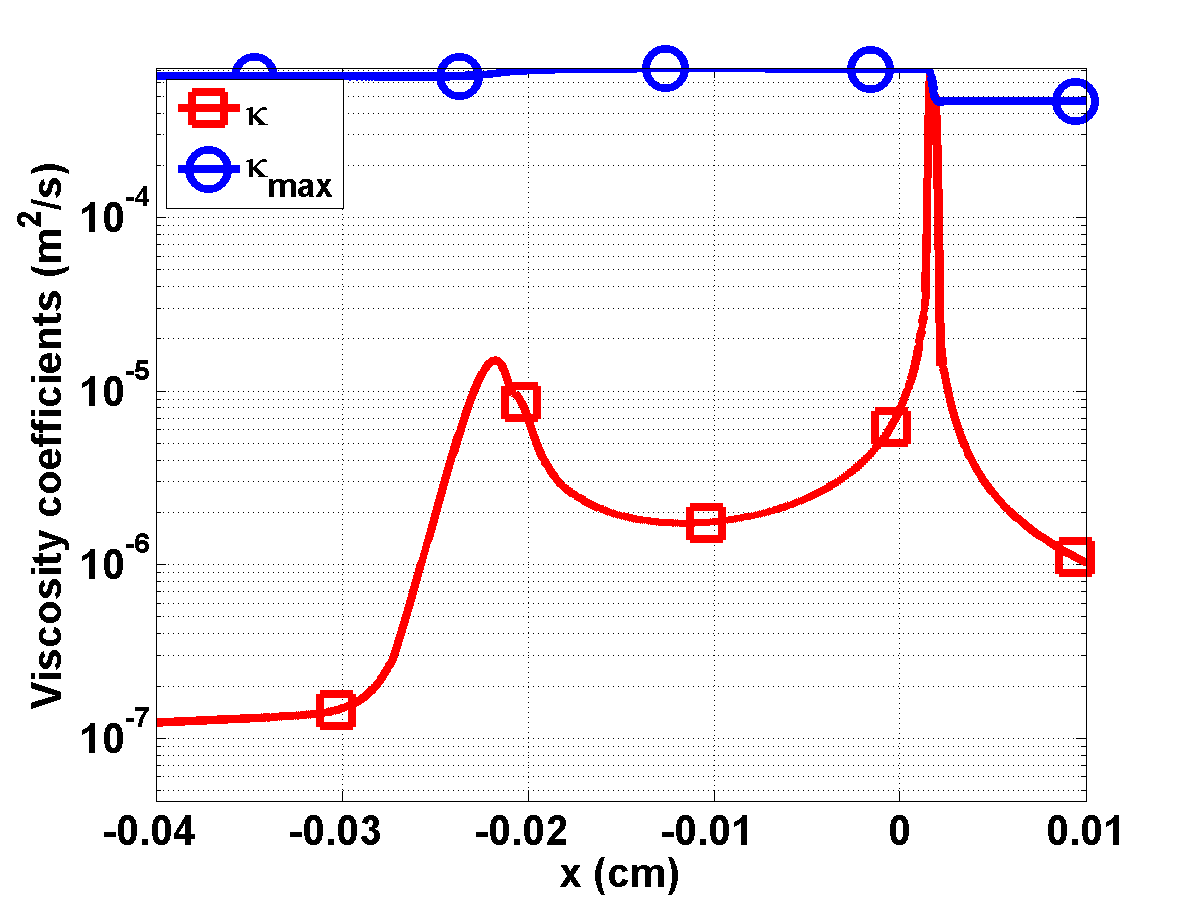
\includegraphics[width=\textwidth]{figs/Mach_5_nel_500_viscosity.png}
        \caption{Viscosity coefficient profiles at steady state for the Mach 5 test.}\label{fig:Mach5_visc}
\end{subfigure}
\end{figure}
%
In \fig{fig:Mach5_temp}, the radiation temperature profile is smooth. The material temperature does not exhibit an embedded hydrodynamic shock but shows a Zeldovich spike. The density profile, \fig{fig:Mach5_dens}, displays a shock located at the same position as the Zeldovich spike of the material temperature profile. The viscosity coefficient $\kappa$ is also peaked in the shock region, as expected. The material and radiation variables do not present any numerical oscillations and match the exact solutions.
%
%%%%%%%%%%%%%%%%%%%%%%%%%%%%%%%%%%%%%%%%%%%%%%%%%%%%%%%%%%%%%%%%%%%%%%%%%%%%%
%%%%%%%%%%%%%%%%%%%%%%%%%%%%%%%%%%%%%%%%%%%%%%%%%%%%%%%%%%%%%%%%%%%%%%%%%%%%%
\section{Conclusions and future work}\label{sec:conclusion}
%%%%%%%%%%%%%%%%%%%%%%%%%%%%%%%%%%%%%%%%%%%%%%%%%%%%%%%%%%%%%%%%%%%%%%%%%%%%%
%%%%%%%%%%%%%%%%%%%%%%%%%%%%%%%%%%%%%%%%%%%%%%%%%%%%%%%%%%%%%%%%%%%%%%%%%%%%%
%
In this paper, we have demonstrated the the viscous regularization, previously derived
for the hyperbolic portion of the non-equilibrium grey radiation hydrodynamic equations,
is fully compatible with the full grey radiation hydrodynamic equations, i.e., when
relaxation source terms and diffusion terms are included in the derivation. That is to say that we have
proven that the proposed viscous regularization of the grey radiation hydrodynamic equations
is entropy-minimum satisfying. 1-D numerical results were presented for a Mach-5 test case.

This regularization has intrinsic mathematical properties of interest for the development of numerical scheme
(e.g., stabilization of numerical discretization schemes by letting the viscosity coefficients be proportional 
to the entropy residual, as in the entropy-viscosity method \cite{jlg1})
and we envision possible applications to larger scale numerical simulations of radiation hydrodynamic processes.

%%%%%%%%%%%%%%%%%%%%%%%%%%%%%%%%%%%%%%%%%%%%%%%%%%%%%%%%%%%%%%%%%%%%%
\setlength{\baselineskip}{12pt}

\bibliographystyle{mc2015}
\bibliography{mybibfile}



\end{document}
